\documentclass[hyperref=colorlinks]{beamer}
\mode<presentation>
\usetheme{iclpt}
\setbeamertemplate{navigation symbols}{}
\setbeamertemplate{headline}{
\begin{beamercolorbox}[leftskip=.2cm,rightskip=.2cm,topskip=.2cm,ht=1.1cm,dp=0.1cm,wd=\textwidth]{institute in head/foot}
  
\includegraphics[height=1cm]{icl.pdf}
  \hfill
  
\includegraphics[height=1cm]{../Pics/CMS-Color.pdf}
\end{beamercolorbox}
}
\setbeamertemplate{footline}{
\begin{beamercolorbox}[ht=.55cm,dp=0.4cm,wd=\textwidth,leftskip=.3cm]{author in head/foot}%
  \begin{minipage}[c]{5cm}%
    \usebeamerfont{author in head/foot}
    \insertshortauthor 
    \insertshorttitle
    \end{minipage}\hfill%
  \insertframenumber{} / \pageref{lastframe}
  \hfill
  \begin{minipage}{6cm}
    \hfill
  \end{minipage}
\end{beamercolorbox}%
}

\usepackage{color}
\usepackage{tabularx,colortbl}
\usepackage{graphicx}
\usepackage{pdfpages}
\usepackage{feynmp}
\usepackage{multirow}
\DeclareGraphicsRule{*}{mps}{*}{}
\usepackage{tikz}
\usetikzlibrary{arrows,shapes,backgrounds}
\tikzset{
  invisible/.style={opacity=0},
  visible on/.style={alt={#1{}{invisible}}},
  alt/.code args={<#1>#2#3}{%                                                                                                                                                                                                                
    \alt<#1>{\pgfkeysalso{#2}}{\pgfkeysalso{#3}} % \pgfkeysalso doesn't change the path                                                                                                                                                      
  },
}

\title{\vspace{-0.2cm} Higgs to Invisible MC Comparison}
%\subtitle{This result: HIG-15-012 \\ Contributing analyses: HIG-13-030, HIG-14-038, EXO-12-055}
\author[P. Dunne]{\underline{P. Dunne}, J. Brooke, M. Buckley, B. Penning, J. Tamanas, M. Zgubic}
\titlegraphic{
  \vspace{-0.7cm}
  %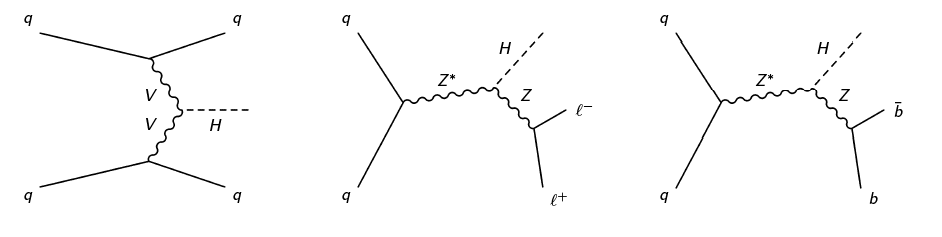
\includegraphics[width=\textwidth]{TalkPics/invcomb021213/feyndiags}
%% \begin{fmfgraph*}(100,70)
%%         \fmfleft{i1,i2}
%%         \fmfright{o1,o2,o3}
%%         \fmf{fermion}{i1,v1,o1}
%%         \fmf{fermion}{i2,v2,o3}
%%         \fmf{phantom,tension=4/5}{v1,v2}
%%         \fmffreeze
%%         \fmf{photon,label=$W,,Z$}{v1,v3}
%%         \fmf{photon,label=$W,,Z$}{v2,v3}
%%         \fmf{dashes}{v3,o2}
%%         \fmflabel{$q$}{i1}
%%         \fmflabel{$q$}{i2}
%%         \fmflabel{$q$}{o1}
%%         \fmflabel{$q$}{o3}
%%         \fmflabel{$H$}{o2}
%%       \end{fmfgraph*}
}
\date{}
\begin{document}
\begin{fmffile}{phenoplots141015feyndiags}

%TITLE PAGE
\section{Title}
\begin{frame}
  \titlepage
  
\end{frame}

\begin{frame}
  \frametitle{Introduction}
  \scriptsize
  \begin{block}{}
    \begin{itemize}
    \item For HIG-13-030 we used a higgs-portal model to set limits on dark matter
    \item This is wrong due to cross-section going to infinity as mass goes to zero
    \item Working with theorists at Rutgers to interpret VBF H$\rightarrow$inv search in several robust BSM dark matter models
    \end{itemize}
  \end{block}
  \centering
  \begin{tikzpicture}
    \node[anchor=south west,inner sep=0] (image) at (0,0) {    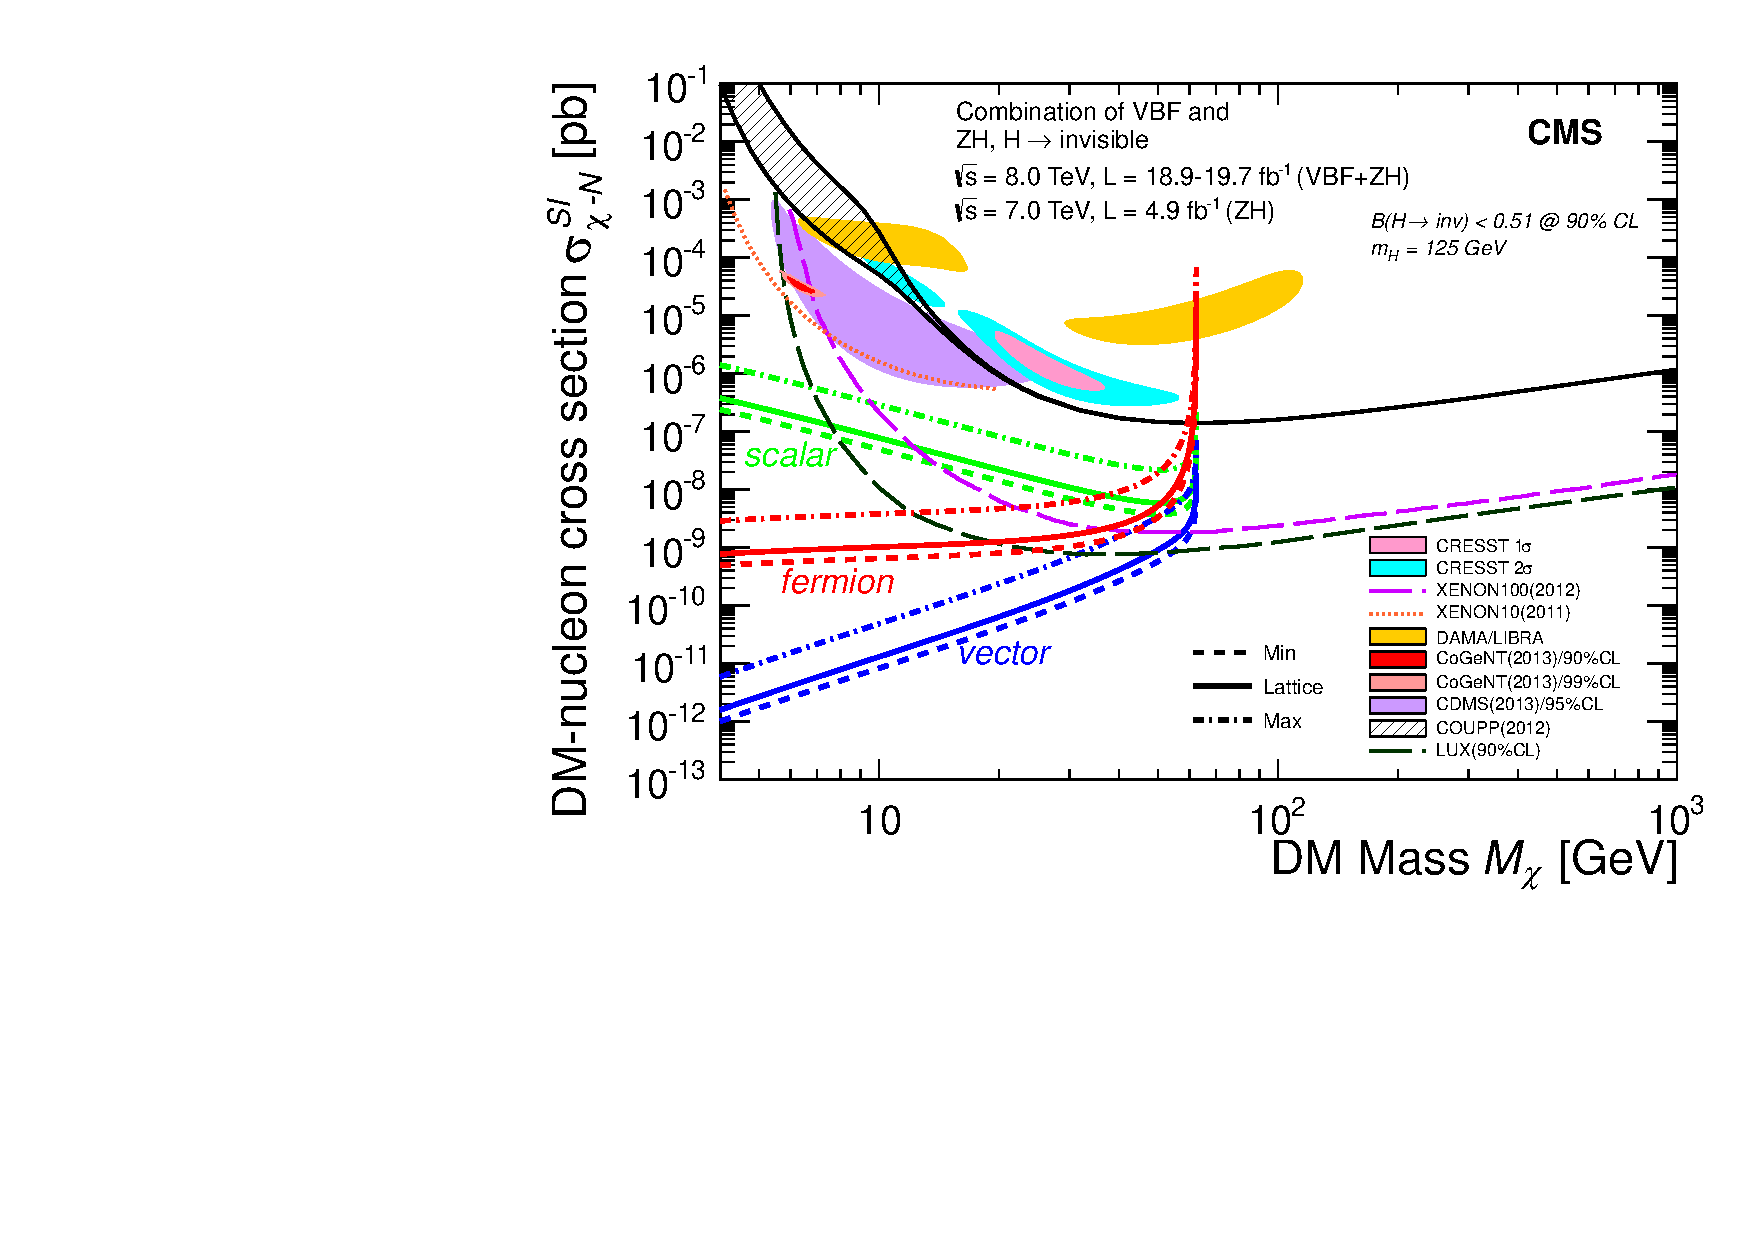
\includegraphics[clip=true,trim=0 0 0 0, width=.6\textwidth]{TalkPics/panicpics/dmlimit.pdf}    };
    \begin{scope}[x={(image.south east)},y={(image.north west)}]
      \draw[red,ultra thick] (0.,0.) -- (1,1);
      \draw[red,ultra thick] (0.,1.) -- (1,0);
    \end{scope}
  \end{tikzpicture}
\end{frame}

\begin{frame}
  \frametitle{Plan for Sample Production}
  \scriptsize
  \begin{block}{}
    \begin{itemize}
    \item The theorists have generated Madgraph samples for several models (SM, EFT, 2HDM, Higgs portal without problems from before) hadronised with pythia
    \item We process them through delphes detector simulation
    \item We then use the scorpion framework to get yields for the models
    \end{itemize}
  \end{block}
\end{frame}

\begin{frame}
  \frametitle{Validation}
  \scriptsize
  \begin{block}{}
    \begin{itemize}
    \item We have SM Higgs to invisible samples generated at 8 TeV with madgraph processed through delphes
    \item[-] Delphes was modified to include met significance
    \item These were compared to CMS samples generated with Powheg and CMS fullsim
    \item Compare yields through cutflow starting at met significance$>3$, $\Delta\eta_{jj}>3.6$
    \end{itemize}
    \scriptsize
    \centering
     \begin{tabular}{|l|c|c|}
      \hline
      Cut added & Powheg + CMS yield & Madgraph + Delphes yield \\
      \hline
      $j_{1}p_{T}>50$, $j_{2}p_{T}>45$ & 1351 & 1834 \\
      min$\Delta\phi(j,met)>2.3$ & 649 & 812 \\
      met$>90$ & 624 & 802 \\
      \textcolor{red}{$M_{jj}>1200$} & \textcolor{red}{300} & \textcolor{red}{194} \\
      \textcolor{red}{met significance$>4$} & \textcolor{red}{273} & \textcolor{red}{167} \\
      \hline
    \end{tabular}
     \begin{itemize}
     \item Not very compatible
     \item Mjj cut seems to be the cause of the largest difference
     \end{itemize}
  \end{block}
\end{frame}

\begin{frame}
  \frametitle{Delphes Validation}
  \scriptsize
  \begin{block}{}
    \begin{itemize}
    \item We wanted to check if the differences seen between Madgraph+delphes and Powheg+CMS were from generator or reconstruction
    \item Powheg samples generated with the same config as the CMS samples were processed with delphes
    \item Default pileup in delphes found to be 50
    \item[-] After correcting to 21 Powheg+CMS and Powheg+Delphes yields now match to 10\%
    \end{itemize}
  \end{block}
\end{frame}

%!!CLOSURE TEST STATEMENT PU jet ID
%OUTLINE
\begin{frame}
  \frametitle{Madgraph vs Powheg: Cut Flow}
  \scriptsize
  \begin{block}{}
    \begin{itemize}
    \item Next check is Madgraph vs Powheg
    \item Compare yields cut by cut
    \item Start with $\eta_{j1}\cdot\eta_{j2}<0$, MET significance$>3$, $\Delta\eta_{jj}>3.6$, jet 1 $p_{T}>35$ GeV, jet 2 $p_{T}>35$ GeV, $M_{jj}>700$ GeV, trigger MET$>40$ GeV 
    \item[-] All variables at trigger threshold plus MET significance$>3$ for technical reasons
    \end{itemize}
    \centering
  \end{block}
  \begin{block}{}
    \begin{tabular}{|l|c|c|}
      \hline
      Cut added & Madgraph + Delphes & Powheg + Delphes \\
      \hline
      Start point & 1552 & 2311 \\
      jet 1 $p_{T}>50$ GeV, jet 2 $p_{T}>45$ GeV & 1203 & 1834 \\
      MET$>90$ GeV & 1170 & 1793 \\
      $M_{jj}>1200$ GeV & 412 & 689 \\
      MET significance$>4$ & 315 & 519 \\
      min$\Delta\phi(j,MET)>2.3$ & 143 & 248 \\
      \hline
    \end{tabular}
  \end{block}
\end{frame}

\begin{frame}
  \frametitle{Madgraph vs Powheg: Efficiencies}
  \scriptsize
  \begin{block}{}
    \begin{itemize}
    \item Compare efficiencies of last cut cut by cut (numbers shown are efficiencies)
    \item Start with $\eta_{j1}\cdot\eta_{j2}<0$, MET significance$>3$, $\Delta\eta_{jj}>3.6$, jet 1 $p_{T}>35$ GeV, jet 2 $p_{T}>35$ GeV, $M_{jj}>700$ GeV, trigger MET$>40$ GeV 
    \item[-] All variables at trigger threshold plus MET significance$>3$ for technical reasons
    \item Efficiencies are very similar
    \item Events that make it to the first step are behaving like they should
    \end{itemize}
    \centering
  \end{block}
  \begin{block}{}
    \begin{tabular}{|l|c|c|}
      \hline
      Cut added & Madgraph + Delphes & Powheg + Delphes \\
      \hline
      jet 1 $p_{T}>50$ GeV, jet 2 $p_{T}>45$ GeV & 0.78 & 0.79 \\
      MET$>90$ GeV & 0.97 & 0.98 \\
      $M_{jj}>1200$ GeV & 0.35 & 0.38 \\
      MET significance$>4$ & 0.76 & 0.75 \\
      min$\Delta\phi(j,MET)>2.3$ & 0.45 & 0.48 \\
      \hline
    \end{tabular}
  \end{block}
\end{frame}


\begin{frame}
  \frametitle{Compare Distributions}
  \scriptsize
  \begin{block}{}
    \begin{itemize}
    \item Use looser selection to look for differences in distributions between Powheg and Madgraph
    \item All plots are normalised to same number of events
    \item Selection: 2 pf jets $p_{T}>30$ GeV
    \item Very different Mjj shape
    \end{itemize}
  \end{block}
  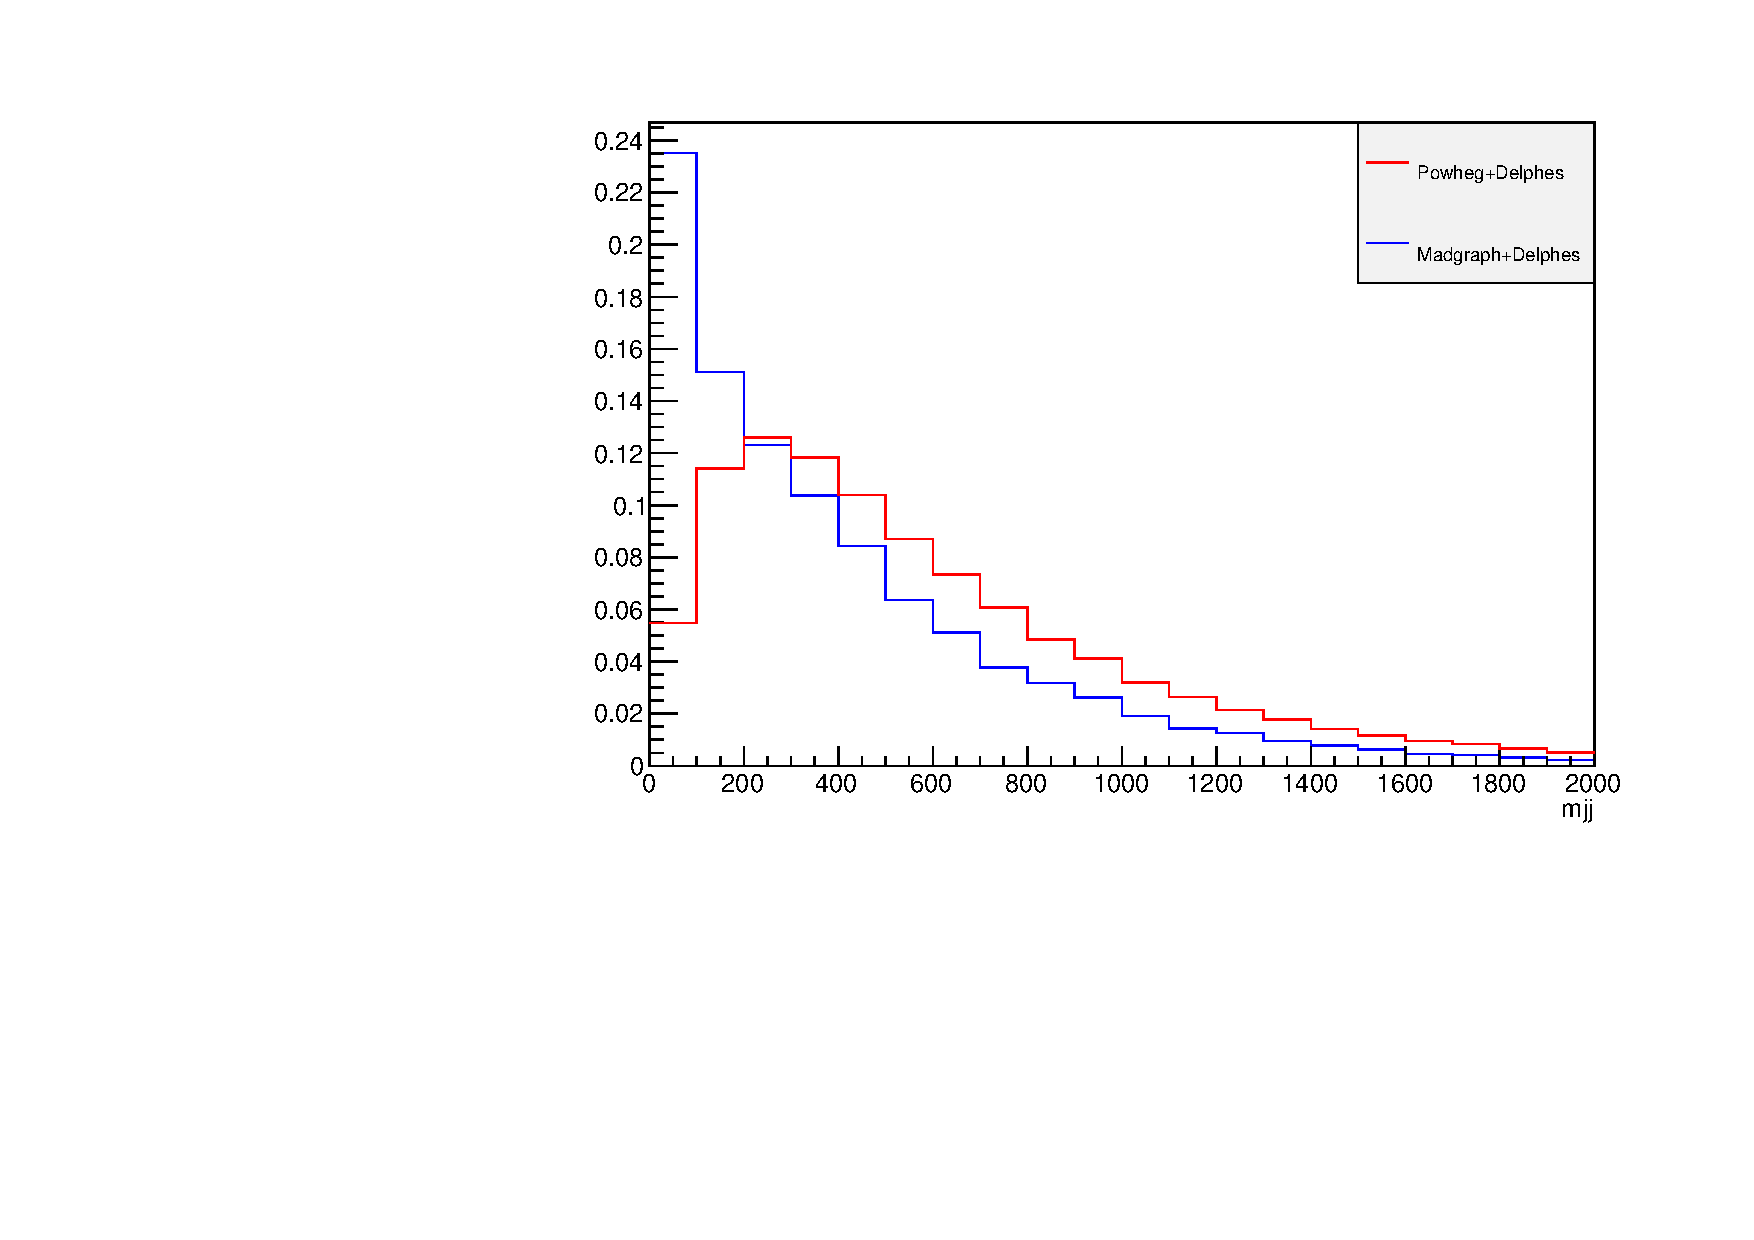
\includegraphics[width=.5\textwidth]{TalkPics/phenoplots281015/mjj_norm.pdf}
  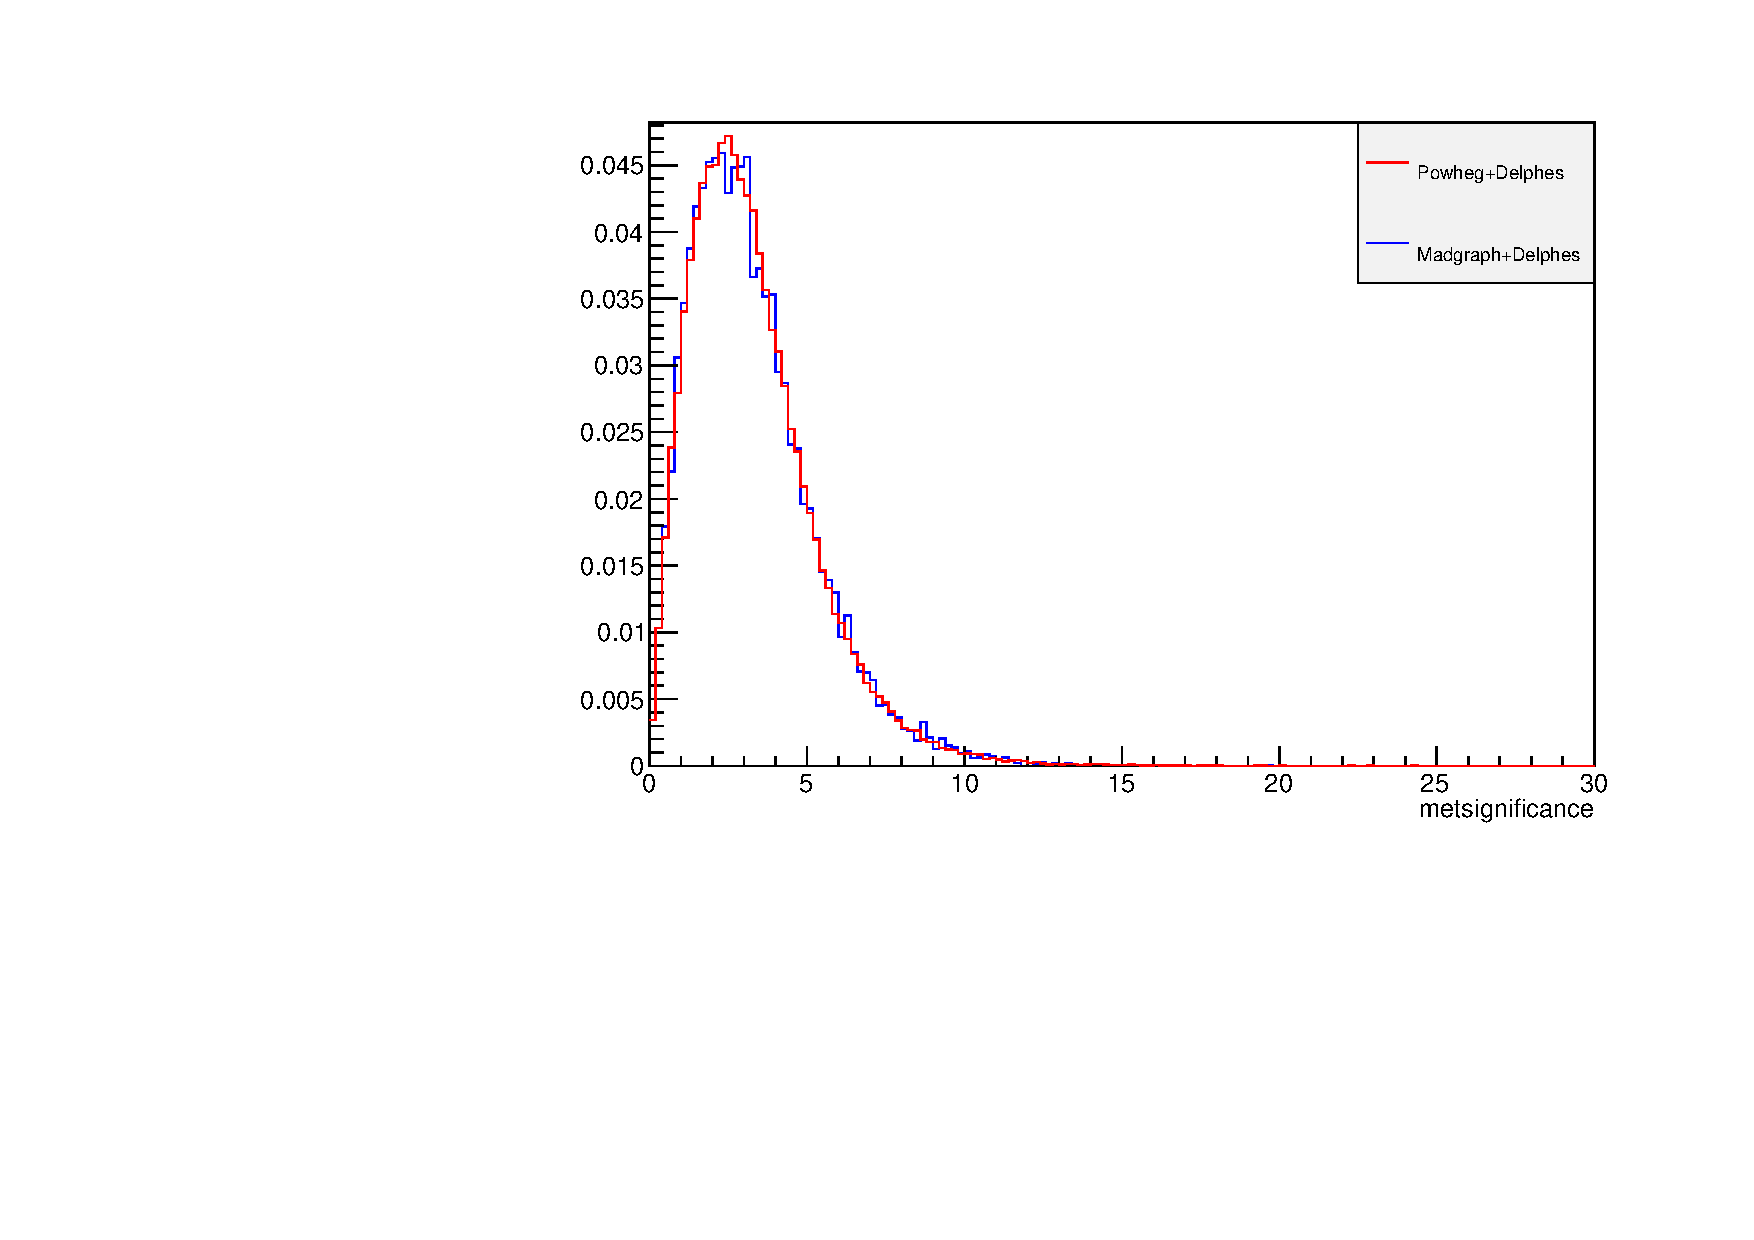
\includegraphics[width=.5\textwidth]{TalkPics/phenoplots281015/metsignificance_norm.pdf}
    
\end{frame}

\begin{frame}
  \frametitle{Compare Distributions}
  \scriptsize
  \begin{block}{}
    \begin{itemize}
    \item Use looser selection to look for differences in distributions between Powheg and Madgraph
    \item All plots are normalised to same number of events
    \item Selection: 2 pf jets $p_{T}>30$ GeV
    \item Very non-VBF like events evident in $\Delta\eta_{jj}$
    \end{itemize}
  \end{block}
  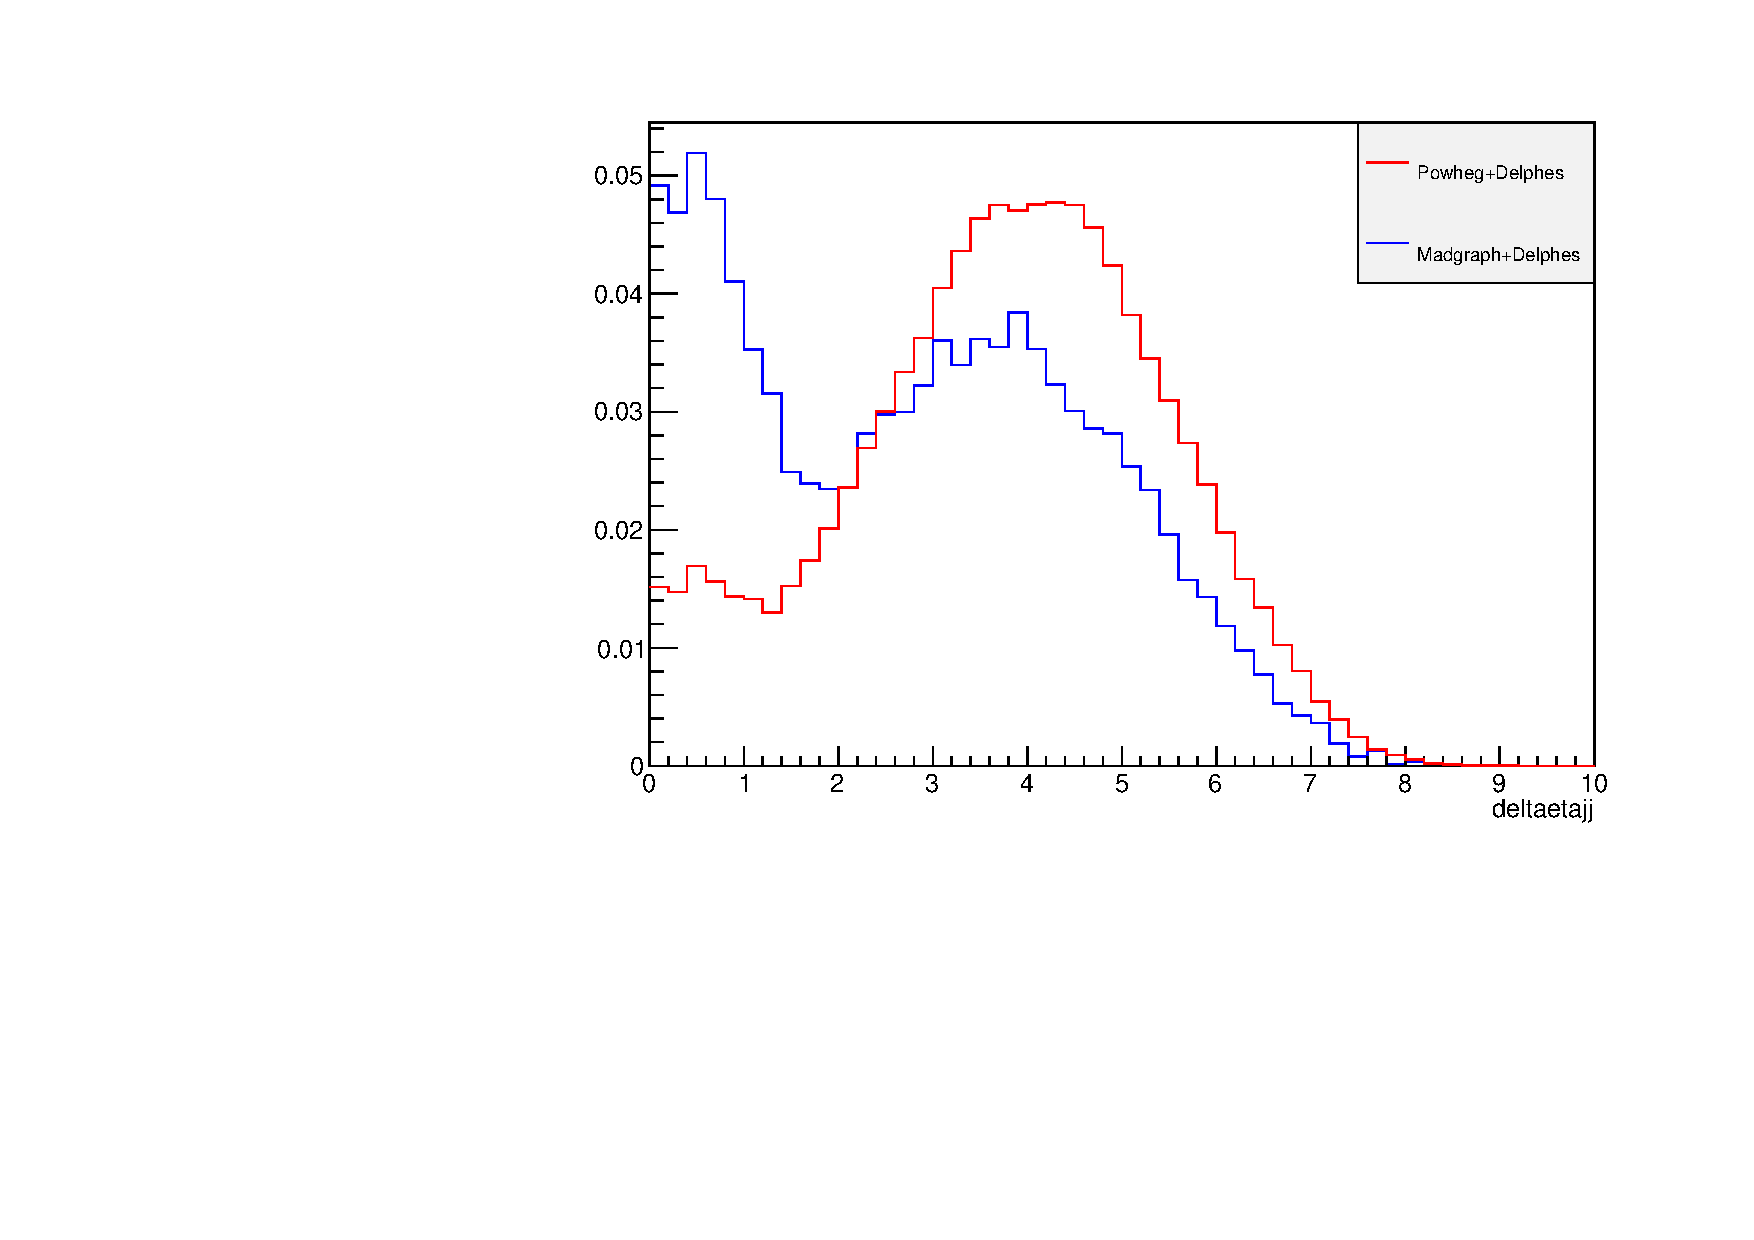
\includegraphics[width=.5\textwidth]{TalkPics/phenoplots281015/deltaetajj_norm.pdf}
  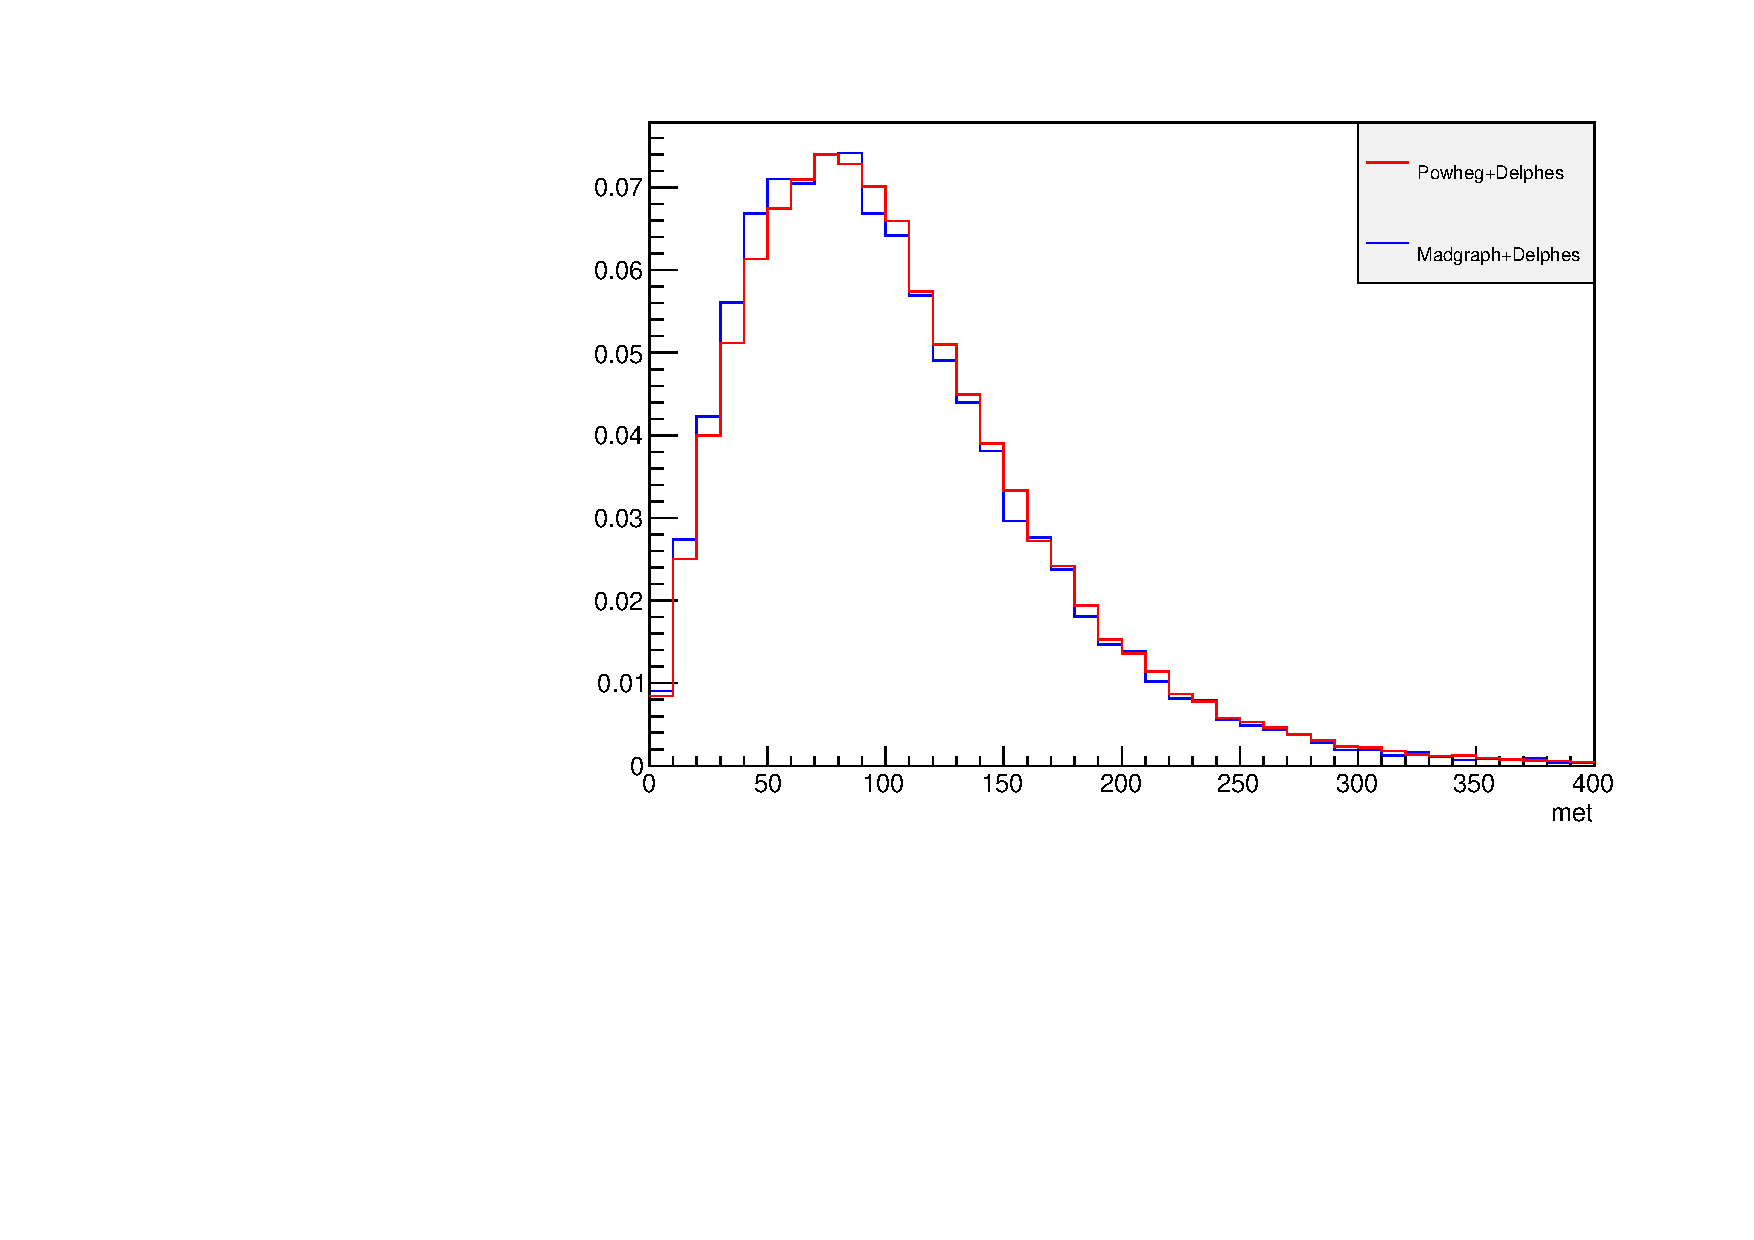
\includegraphics[width=.5\textwidth]{TalkPics/phenoplots281015/met_norm.pdf}
 
\end{frame}

\begin{frame}
  \frametitle{Compare Distributions}
  \scriptsize
  \begin{block}{}
    \begin{itemize}
    \item Use looser selection to look for differences in distributions between Powheg and Madgraph
    \item All plots are normalised to same number of events
    \item Selection: 2 pf jets $p_{T}>30$ GeV
    \end{itemize}
  \end{block}
  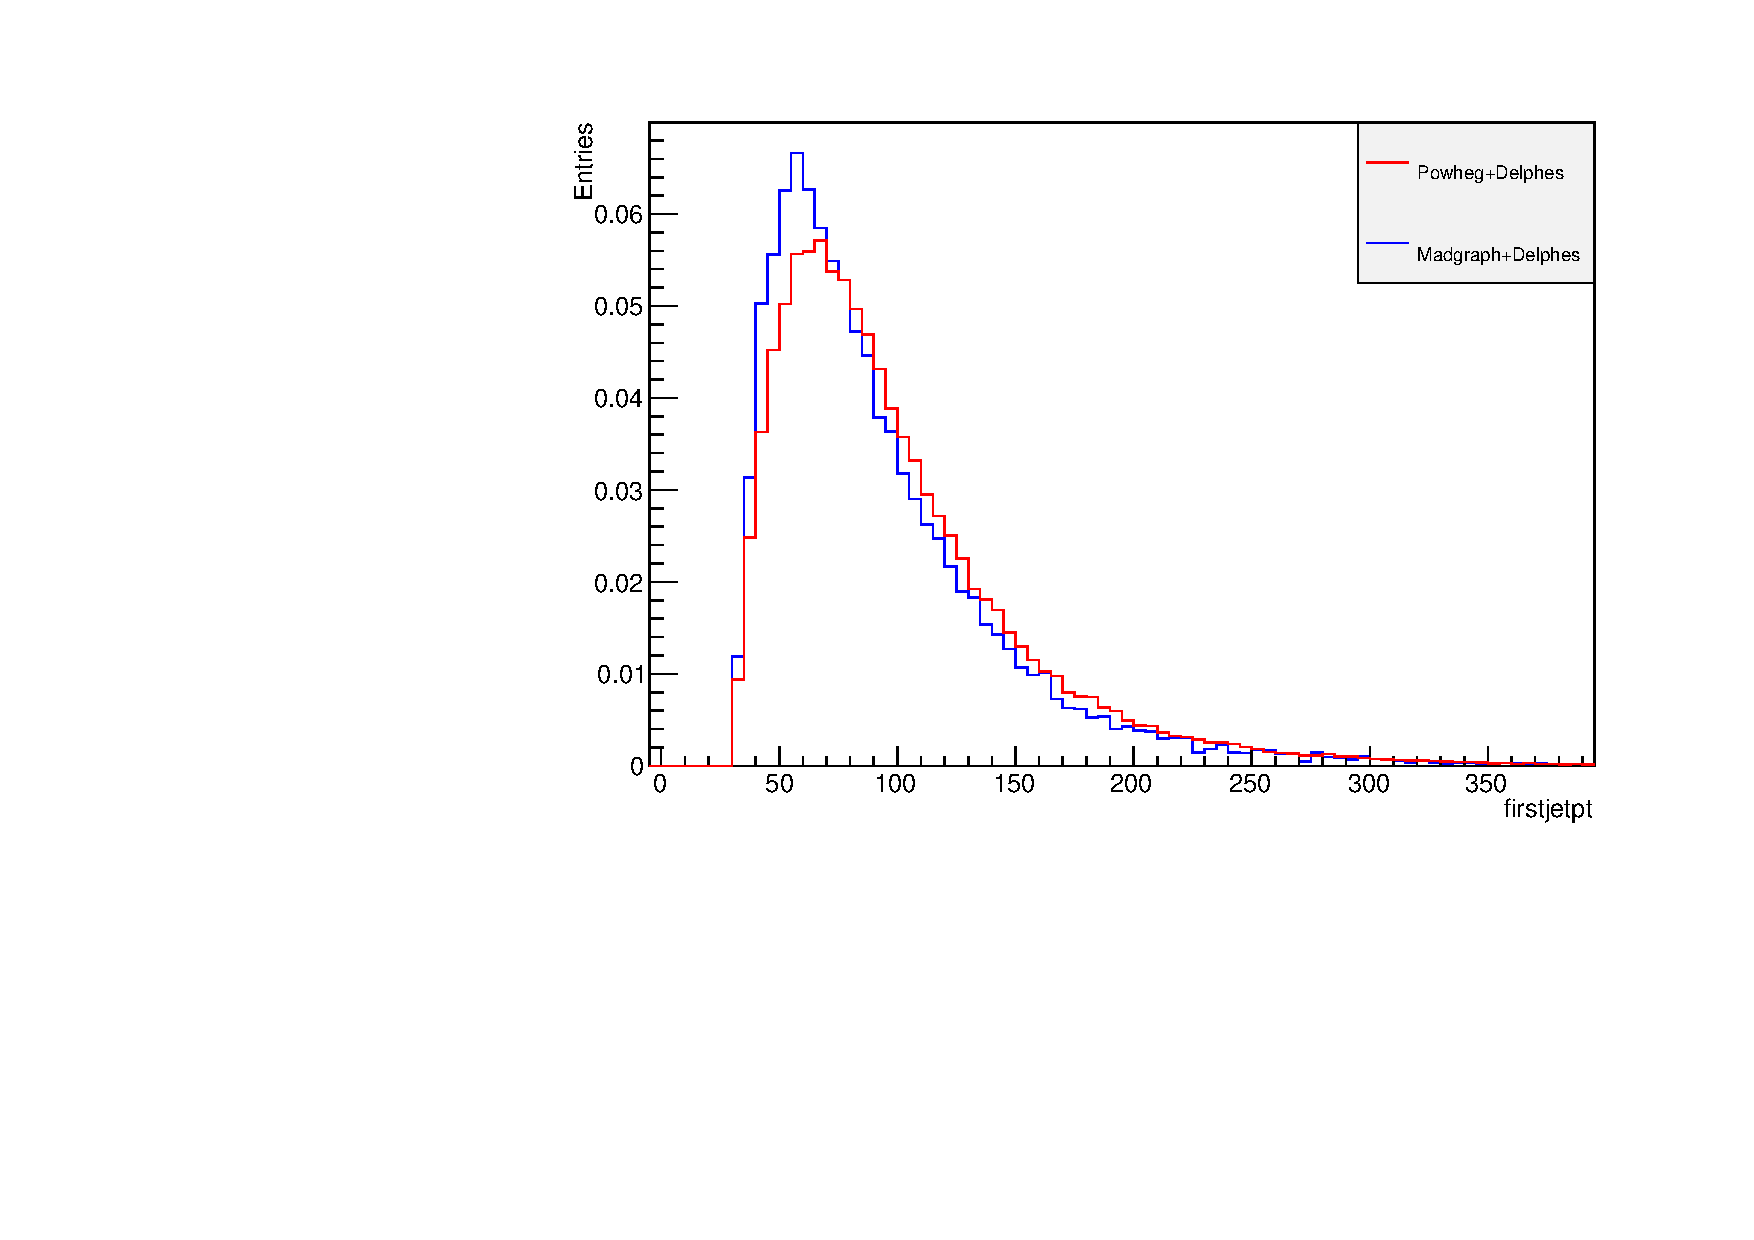
\includegraphics[width=.5\textwidth]{TalkPics/phenoplots281015/firstjetpt_norm.pdf}
  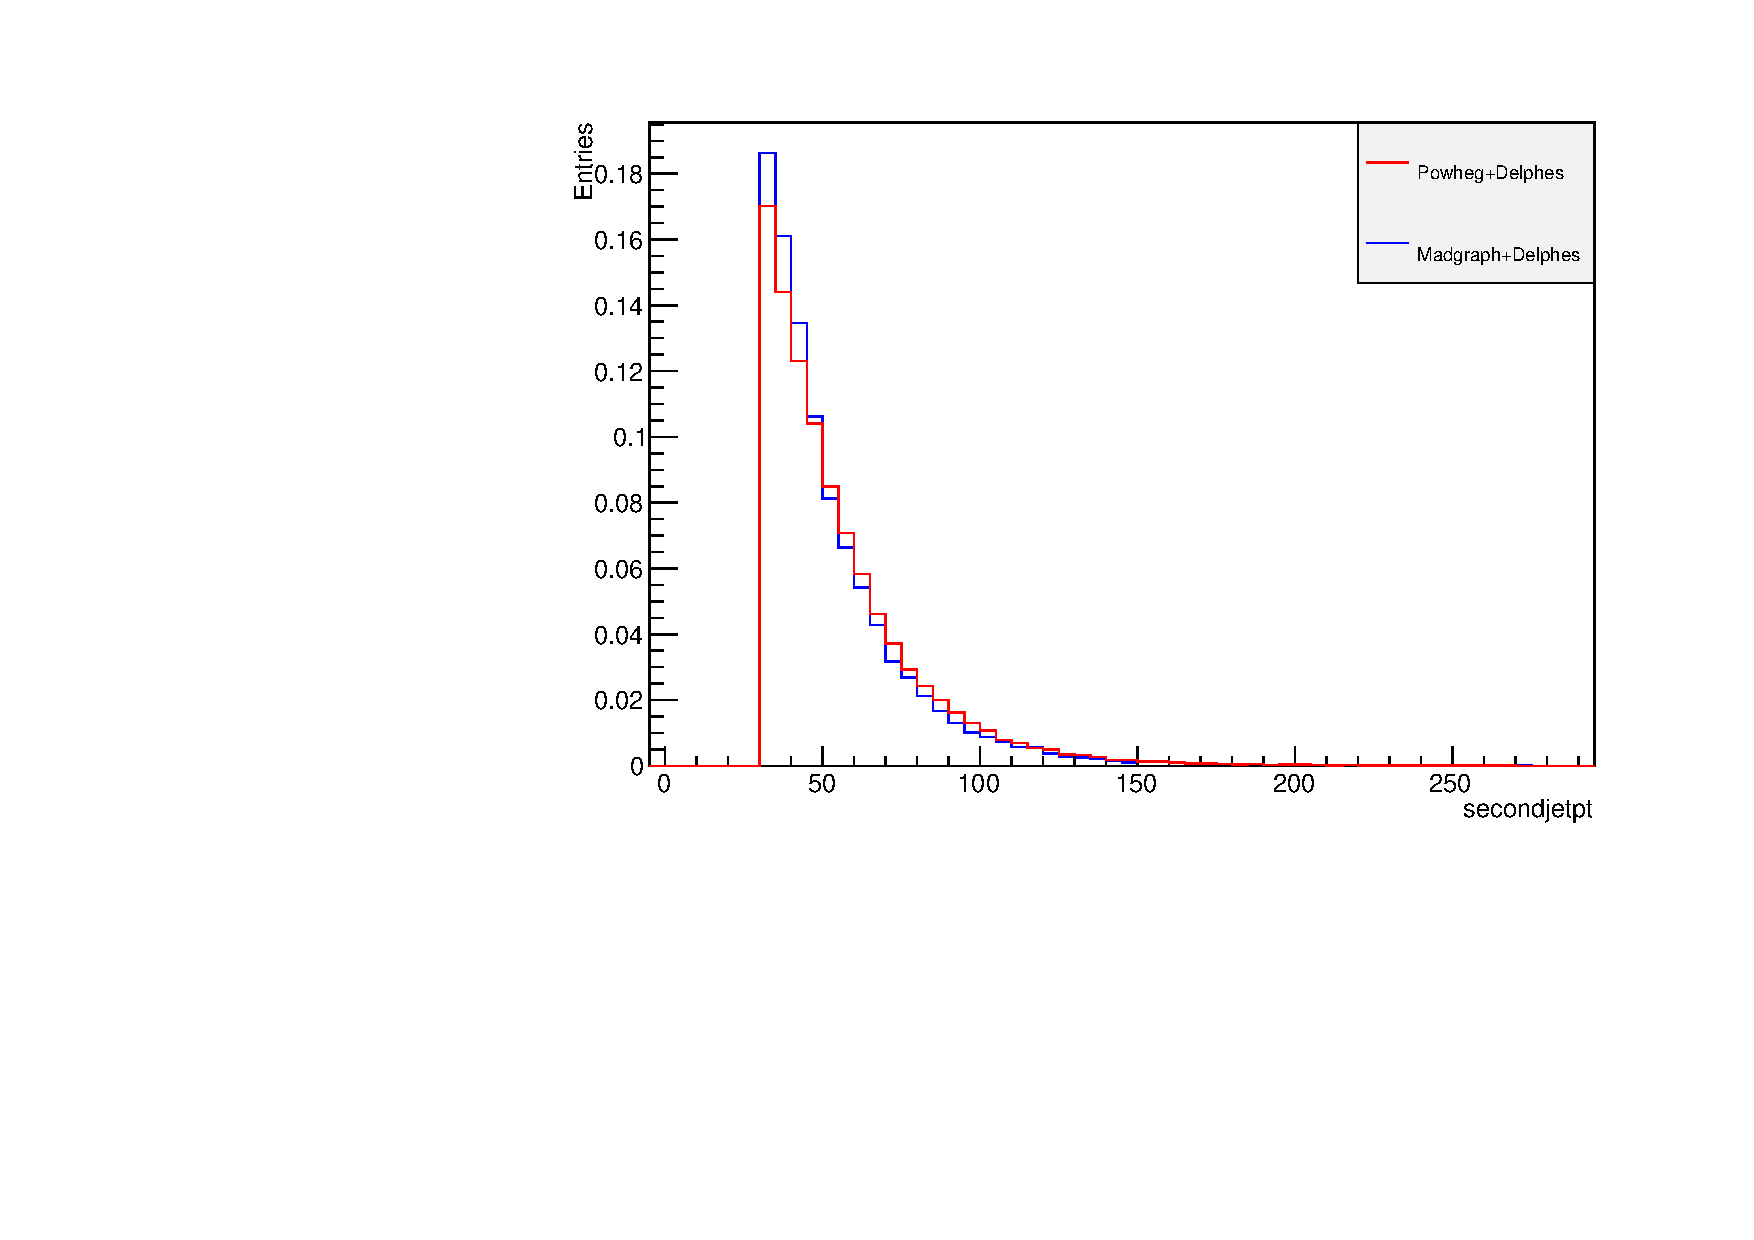
\includegraphics[width=.5\textwidth]{TalkPics/phenoplots281015/secondjetpt_norm.pdf}
    
\end{frame}


\begin{frame}
  \frametitle{Compare Distributions}
  \scriptsize
  \begin{block}{}
    \begin{itemize}
    \item Use looser selection to look for differences in distributions between Powheg and Madgraph
    \item All plots are normalised to same number of events
    \item Selection: 2 pf jets $p_{T}>30$ GeV
    \end{itemize}
  \end{block}
  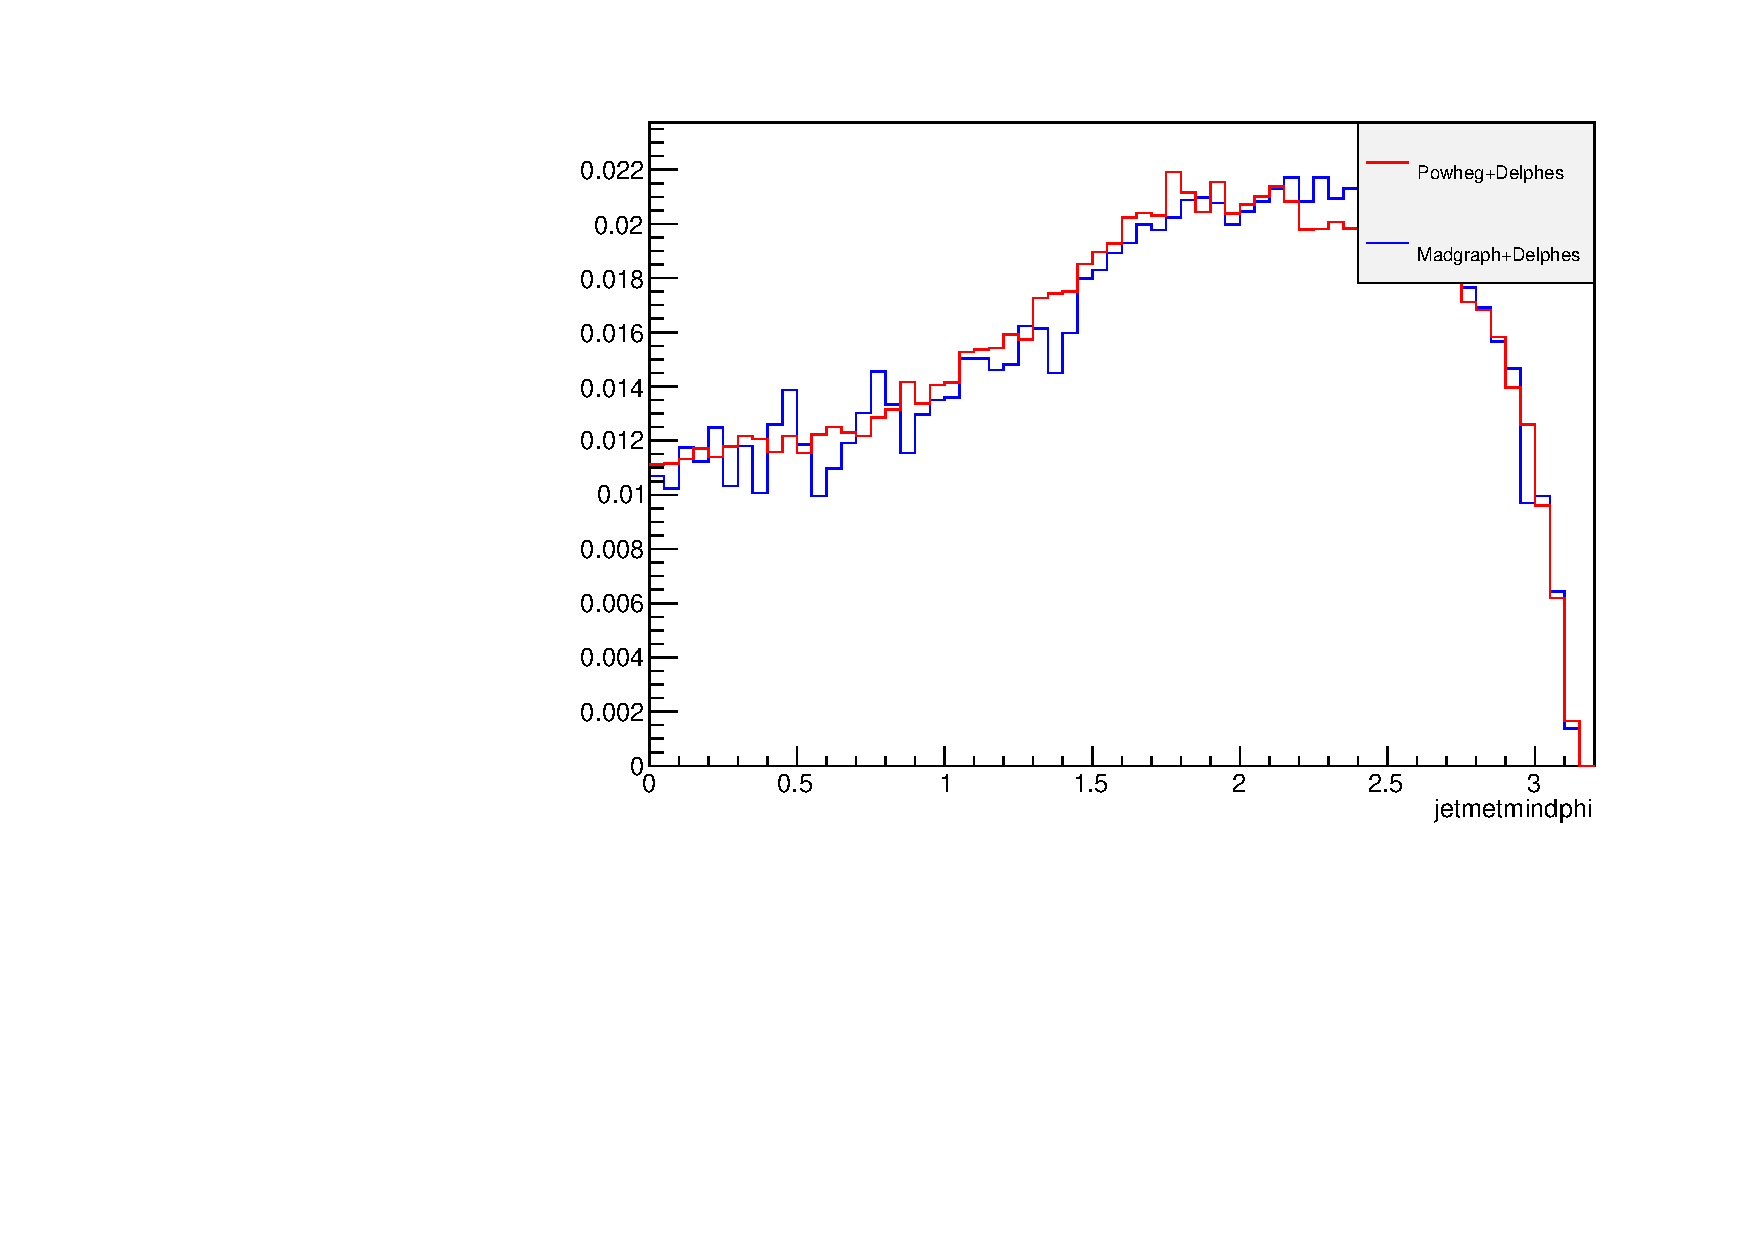
\includegraphics[width=.5\textwidth]{TalkPics/phenoplots281015/jetmetmindphi_norm.pdf}
  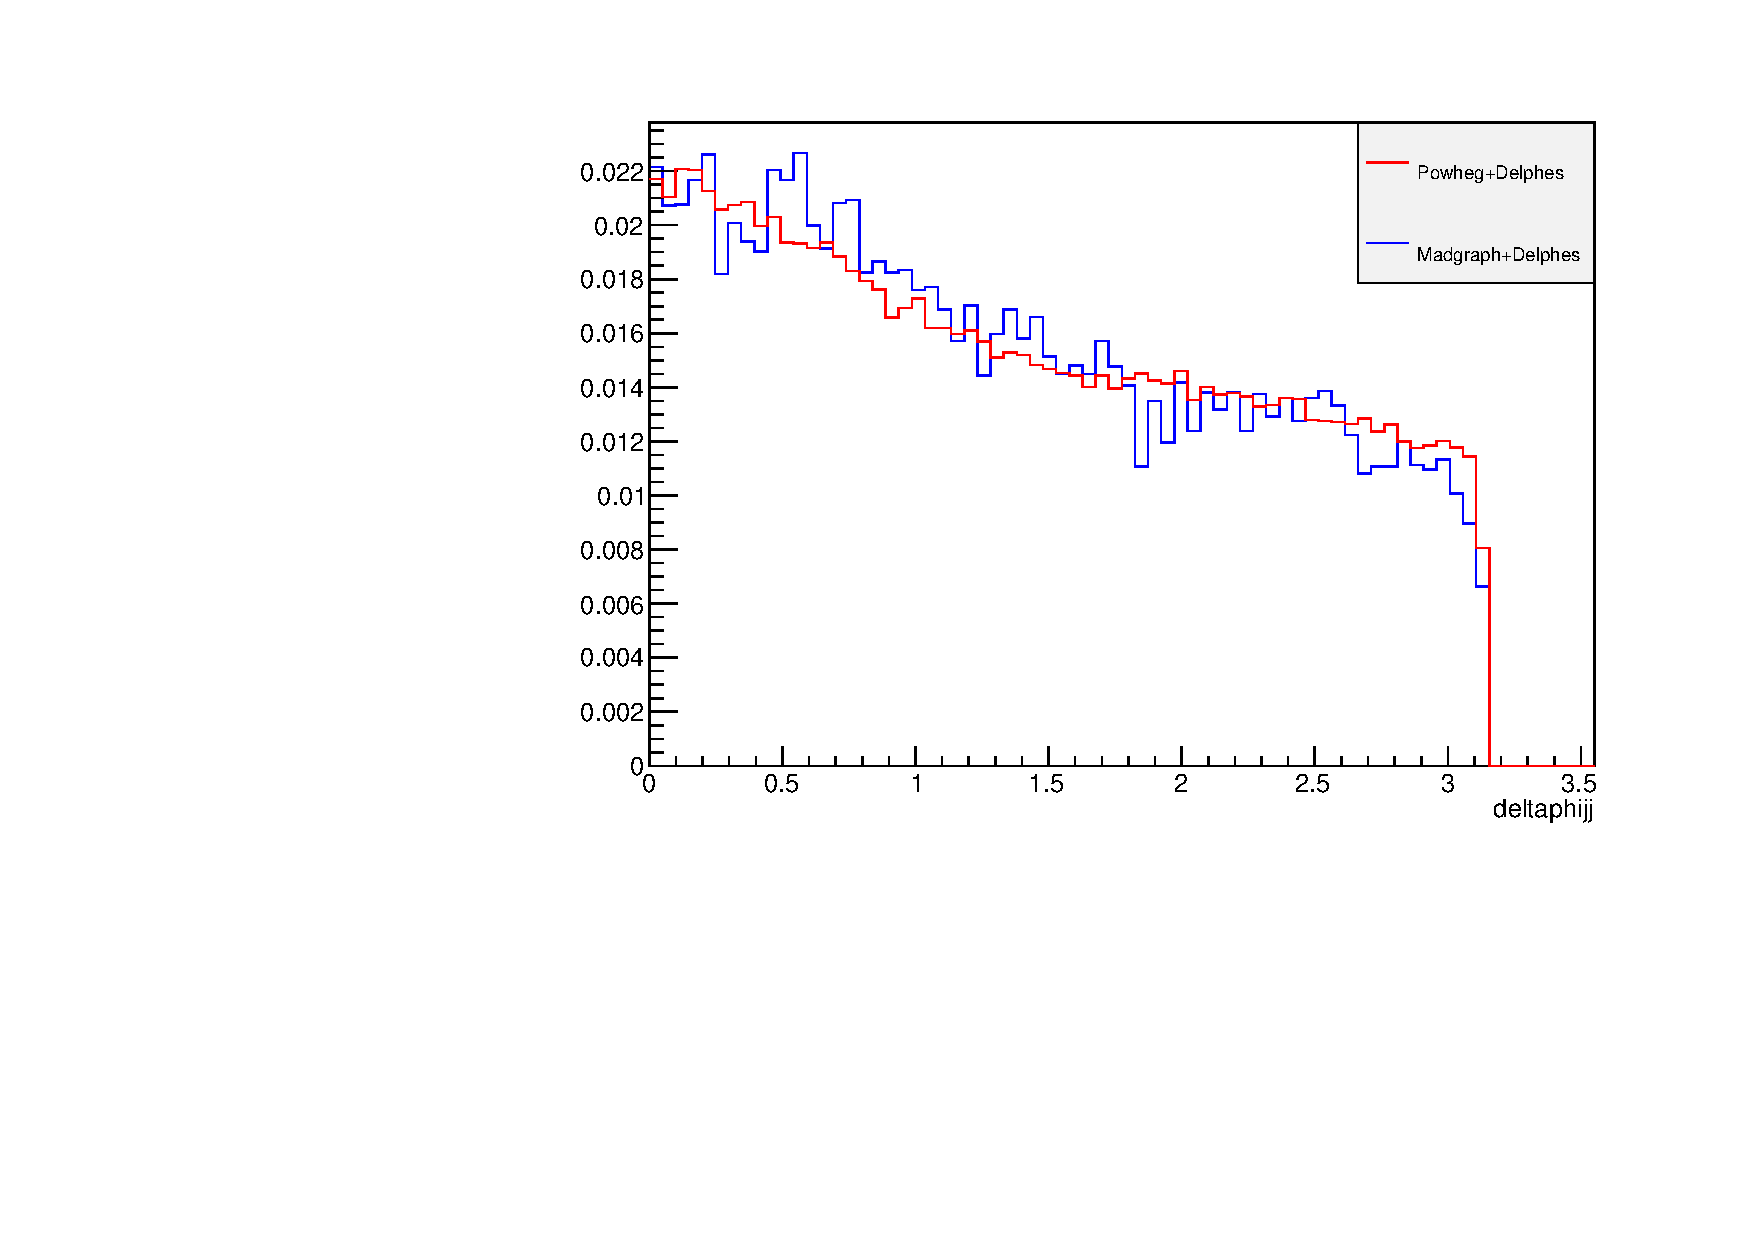
\includegraphics[width=.5\textwidth]{TalkPics/phenoplots281015/deltaphijj_norm.pdf}
 
\end{frame}

\begin{frame}
  \frametitle{Problem Resolved}
  \scriptsize
  \begin{block}{}
    \begin{itemize}
    \item On discussion with theorists VH production is same EWK order as VBF and therefore present in Madgraph samples
    \item We expect no VH events to pass our full selection so changing normalisation cross-section should resolve differences
    \end{itemize}
    \begin{tabular}{|l|c|c|}
      \hline
      Cut added & Madgraph + Delphes & Powheg + Delphes \\
      \hline
      Start point & 2653 & 2311 \\
      jet 1 $p_{T}>50$ GeV, jet 2 $p_{T}>45$ GeV & 2056 & 1834 \\
      MET$>90$ GeV & 2000 & 1793 \\
      $M_{jj}>1200$ GeV & 704 & 689 \\
      MET significance$>4$ & 539 & 519 \\
      min$\Delta\phi(j,MET)>2.3$ & 244 & 248 \\
      \hline
    \end{tabular}
    \begin{itemize}
    \item Agreement now very good
    \end{itemize}
  \end{block}
\end{frame}

\begin{frame}
  \frametitle{Limits}
  \scriptsize
  \begin{block}{}
    \begin{itemize}
    \item Non-CMS publication so we cannot use full datacard with internal correlation and uncertainty information
    \item I have made a datacard using only the information publicly available in the PAS
    \item Compare limits:
    \end{itemize}
    \centering
    \begin{tabular}{|l|c|c|}
      \hline
      Card & Signal estimate used & Observed (expected) limit \\
      \hline
      CMS & CMS & 57(40) \\
      CMS & CMS & 63(45) \\
      Public info & MG+Delphes & 58(42) \\
      Public info & MG+Delphes & 65(47) \\
      \hline
    \end{tabular}
    \begin{itemize}
    \item For MG+Delphes signal estimate I've assumed the same errors and the same proportion of ggH contamination
    \item Using public info only doesn't change limit much
    \item Different signal estimate leads to agreement at 10\% level
    \end{itemize}
  \end{block}
\end{frame}

\begin{frame}
  \frametitle{Summary}
  \label{lastframe}
  \begin{block}{}
    \scriptsize
    \begin{itemize}
    \item We have a well validated software chain to emulate the CMS VBF H$\rightarrow$invisible parked analysis
    \item We will now process the BSM samples generated by the theorists
    \item We will also extrapolate to 13 TeV to estimate future sensitivity
    \item[-] Scale backgrounds by parton luminosity, systematics constant/$\sqrt{\mathcal{L}}$
    \end{itemize}
  \end{block}
  \centering
  %!!INCLUDE A RUN 2 PLOT
\end{frame}

%UPDATED BACKUP
\begin{frame}
  \frametitle{Backup}
\end{frame}

\end{fmffile}
\end{document}
